
\documentclass[8pt]{beamer}
\usepackage[authoryear,round]{natbib}
\usepackage{graphicx}
\usepackage{fancybox}
\usetheme[width=2cm]{Goettingen}
\usepackage[utf8x]{inputenc}
\usepackage[T1]{fontenc}
\usepackage[french]{babel}
\usepackage[small]{caption}
%%%Présentation faite pour le seminaire organisé par ces grand noms du HCCL

\author{Simon}
\title{La Robotique \'Evolutionnaire, un modèle pour étudier la Théorie de l'\'Evolution}
\begin{document}

\begin{frame}
	\titlepage
\end{frame}

\section{La théorie de l'évolution}
\begin{frame}{La théorie darwinienne de l'évolution}
	Chez Darwin:
	\begin{quote}
		Theory of descent with modification by variation and Natural Selection
	\end{quote}

	\vfill

	Deux composantes :
	\begin{itemize}
		\item L'Hypothèse de la sélection naturelle : ``survival of the fittest'' (formulation de Spencer).
		\item Descente avec Modification : variation aléatoire et hérédité.
	\end{itemize}
	Conséquences : une théorie qui explique comment les espèces se modifient \emph{et} se différencient.
\end{frame}

\begin{frame}{Descente avec modifications}
	Nécessité théorie de l'hérédité avec propriétés compatible avec la théorie de Darwin (pagnésèse chez Darwin).
	\newline
	\begin{center}
		\emph{A priori non vrai avec le Mendelism!}\\
		(Mendel = 1/4 A 1/2Aa 1/4 a)
	\end{center}
\end{frame}
\begin{frame}{Hypothèse de la Sélection Naturelle}
	Comment la prouver? 

	
	\begin{itemize}
		\item Analogie avec la Sélection Artificielle.
		\item ``Preuve'' mathématique (statistique) : les biométriciens (1890 - 1916 Pearson, Weldon) mais très peu évident à pour Darwin (critique de Jenkins la plus ``serieuse'' selon lui, cf Gayon).
	\end{itemize}


\end{frame}

\begin{frame}{Théorie synthétique de l'évolution}
	Reconciliation du Mendelisme et de Darwin, la théorie génétique de l'évolution \cite{fisher1930geneticaltheorynaturalselection}. puis la synthèse moderne.
\vfill 
	Mêmes outils mais différentes approches scientifiques.
	\begin{itemize}
		\item Fisher : Idéal Newtonien
		\item Wright : importance des interaction local
	\end{itemize}
	
\end{frame}
\begin{frame}{Niveau et unité de sélection}
	Depuis Wallace et Darwin les interpretations divergent(cf Lloyds SEP). Les avancées scientifiques n'ont pas résolu le problèmes (problèmes reductionnisme, genes mendel = many to many)  
	\vfill
	\begin{beamerboxesrounded}{Différentes questions à différentes echelles}
		Espèce, groupes, individus, gènes qui sont sélectionnés?\\
	        Espèce, groupes, individus, gènes qui sont modifiés?
	\end{beamerboxesrounded}
	\vfill
	Exemple de l'émergence de l'altruisme. Fonctionne parfois avec selection de groupe, parfois sans, dépendance très fortes des paramètres des modèles utilisées.



\end{frame}
\begin{frame}{Approche sémantique des théories}
	Van Frassen
\end{frame}
\section{Robotique \'Evolutionnaire}
\subsection{Histoire}
\begin{frame}{Algorithmique \'Evolutionnaire et Robotique}

	\vfill
	\begin{columns}
		\column{.5\textwidth}
		\begin{figure}[h]
			\begin{center}
				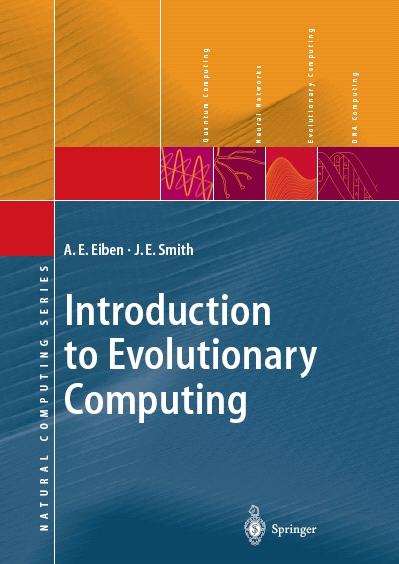
\includegraphics[height=4cm]{images/ec}
			\end{center}
			\caption{\cite{eiben03introductiontoevolutionarycomputing}}
			\label{fig:ec}
		\end{figure} 

		\vfill
		Algoritmique Évolutionaire 1970 : \cite{holland75adaptationnaturalartificialsystem}


		\column{.5\textwidth}

		\begin{figure}[h]
			\begin{center}
				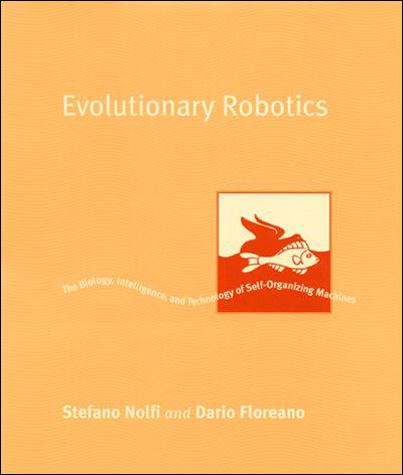
\includegraphics[height=4cm]{images/er}
			\end{center}
			\caption{\cite{nolfi00evolrobobiolintetechselfmach}}
			\label{fig:er}
		\end{figure}

		\vfill
		Robotique Évolutionnaire 1990 : \cite{nolfi00evolrobobiolintetechselfmach}
	\end{columns}
	\vfill

	$\rightarrow$ utiliser Darwin pour concevoir des systèmes artificiel
\end{frame}

\begin{frame}
	Algorithme génétique :
	\begin{figure}
		\centering
		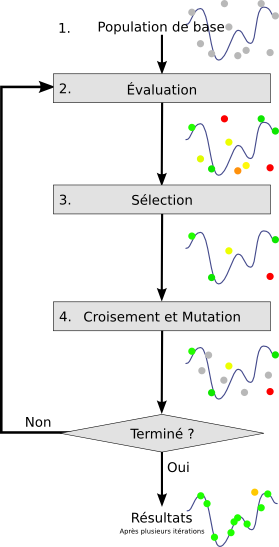
\includegraphics[width=.3\textwidth]{images/AG.png}
		\caption{Exemple d'algorithme génétique (source : wikipedia)}\label{fig:AG}
	\end{figure}
\end{frame}

\begin{frame}
	Test des  niveau de sélection. 
	Sélection des individus en fonction de la fitness du groupe.
	Waibel, Keller et Floreano 2009.
\end{frame}

\begin{frame}
	\bibliographystyle{apalike}
	\bibliography{/home/simon/Documents/biblio/memoireLophiss}
\end{frame}

\end{document}
